% TEMPLATE for Usenix papers, specifically to meet requirements of
%  USENIX '05
% originally a template for producing IEEE-format articles using LaTeX.
%   written by Matthew Ward, CS Department, Worcester Polytechnic Institute.
% adapted by David Beazley for his excellent SWIG paper in Proceedings,
%   Tcl 96
% turned into a smartass generic template by De Clarke, with thanks to
%   both the above pioneers
% use at your own risk.  Complaints to /dev/null.
% make it two column with no page numbering, default is 10 point

% Munged by Fred Douglis <douglis@research.att.com> 10/97 to separate
% the .sty file from the LaTeX source template, so that people can
% more easily include the .sty file into an existing document.  Also
% changed to more closely follow the style guidelines as represented
% by the Word sample file. 

% Note that since 2010, USENIX does not require endnotes. If you want
% foot of page notes, don't include the endnotes package in the 
% usepackage command, below.

% This version uses the latex2e styles, not the very ancient 2.09 stuff.
\documentclass[letterpaper,twocolumn,10pt]{article}
\usepackage{usenix,epsfig, graphicx, subcaption}
\begin{document}

%don't want date printed
\date{}

%make title bold and 14 pt font (Latex default is non-bold, 16 pt)
\title{\Large \bf Scalable Crowd-sourced Live Streaming System}

%for single author (just remove % characters)
\author{
{\rm Anbang Zhao}\\
Carnegie Mellon University\\
5000 Forbes Ave\\
Pittsburgh, PA 15213, USA\\
anbangz@cs.cmu.edu
\and
{\rm Zhuo Chen}\\
Carnegie Mellon University\\
5000 Forbes Ave\\
Pittsburgh, PA 15213, USA\\
zhuoc@cs.cmu.edu
% copy the following lines to add more authors
\and
{\rm Mahadev Satyanarayanan}\\
Carnegie Mellon University\\
5000 Forbes Ave\\
Pittsburgh, PA 15213, USA\\
satya@cs.cmu.edu
} % end author

\maketitle

% Use the following at camera-ready time to suppress page numbers.
% Comment it out when you first submit the paper for review.
\thispagestyle{empty}


\subsection*{Abstract}

We propose a scalable system for Internet scale crowd-sourced live streaming video broadcasting from wearable devices, like Google Glass and smart watches. Instead of the widely used centralized system architecture which inevitably face single point bottlenecks, our approach uses a decentralized architecture on cloudlets. We construct an overlay tree on top of cloudlets connected via wide area network (WAN) and do application layer multicast (ALM) on those nodes which effectively reduced bandwidth consumption from linear to client number to linear to cloudlet number. Furthermore, to make this system work, each cloudlet node can just send one copy of the stream, which effectively solves the single node bottleneck. In the Internet scale, there might be hundreds or thousands of cloudlets serving the same stream, our system can tolerate possible cloudlet failures and reconstruct the tree structure within a short period of time. Our experiments show that our system can effectively reduce bandwidth consumption on WAN and keep the same video quality.

\subsection*{Keywords}

mobile computing, application layer multicast, cloud computing, cloudlet, Google Glass

\section{Introduction}

Wearable devices with a camera on it has becoming more and more popular over the past years. Go Pro sold 2.3 million devices in the year of 2012 and Go Pro users can easily upload their Go Pro videos to their favorite video websites (e.g. YouTube) through their mobile devices. Google launched the famous Google Glass in 2012 and it soon became a star in the technology world. Galaxy Gear and Apple Watch are more recent such kind of products that draw much attention from the world. With these kind of technology products, to capture and broadcast a first-person viewpoint video just requires the user to press a button or touch the screen. People can do what they intend to do without interferences brought by wearing those devices and doing video capturing. A good example of this is the first-person hiking videos captured by Go Pro on YouTube. They have good resolution and gives viewers a better experience. Another example is JustinTV, which turned into Twitch and was acquired by Amazon with 1 billion dollars. It was famous for providing first-person videos of good game players and people love to watch it.

\begin{figure}[t]
\begin{center}
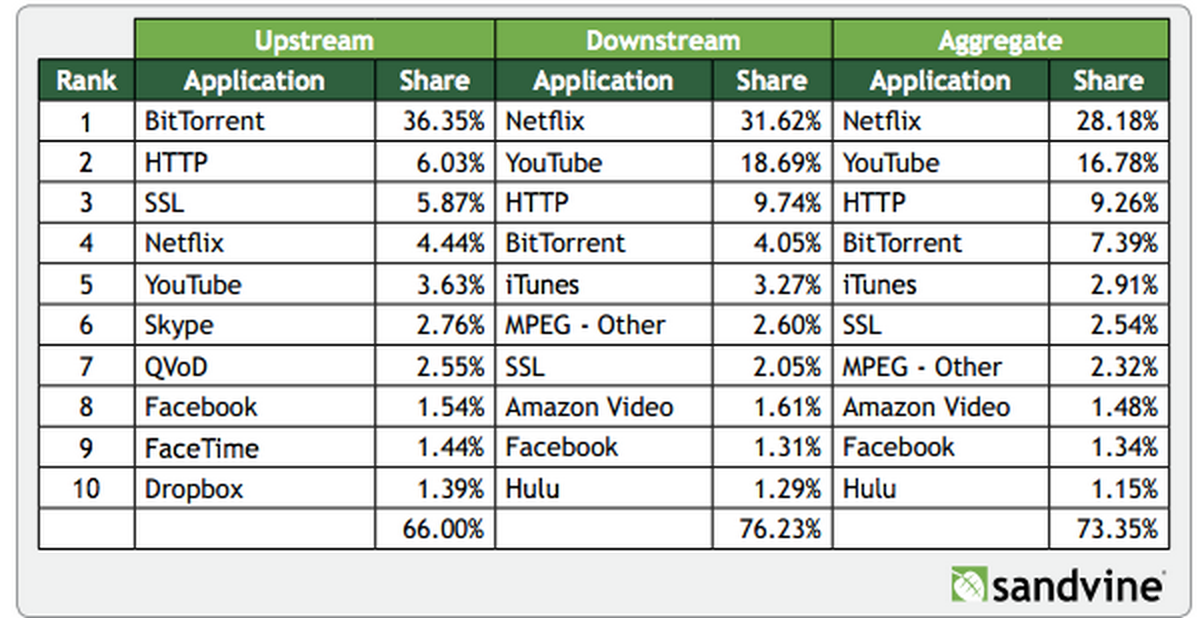
\includegraphics[scale=0.3]{pic/bandwidth_rank.png}
\end{center}
\caption{US bandwidth consumption (from sandvine)}
\end{figure}

We believe video broadcasting is the more intuitive and vivid way of communication and emotion sharing and more and more people will use this kind of service. But this service comes with a big price, Internet bandwidth in both uploading and downloading. Video stream is already the biggest consumer on the Internet. As shown in Figure 1, Netflix and Youtube consume about half the downloading bandwidth in the US. We can anticipate an even greater download bandwidth consumption if those live streaming videos are available. Besides, the upload bandwidth consumption will increase even more than the download bandwidth consumption. Currently, uploading video is not much more troublesome than watch a video. However, in the near future, it will become as easy because of the all the smart hardwares. At that time, the bandwidth bottleneck of the current video system will be more severe because content distribution network (CDN) will not help neither. 



\begin{figure}[h]
\begin{center}
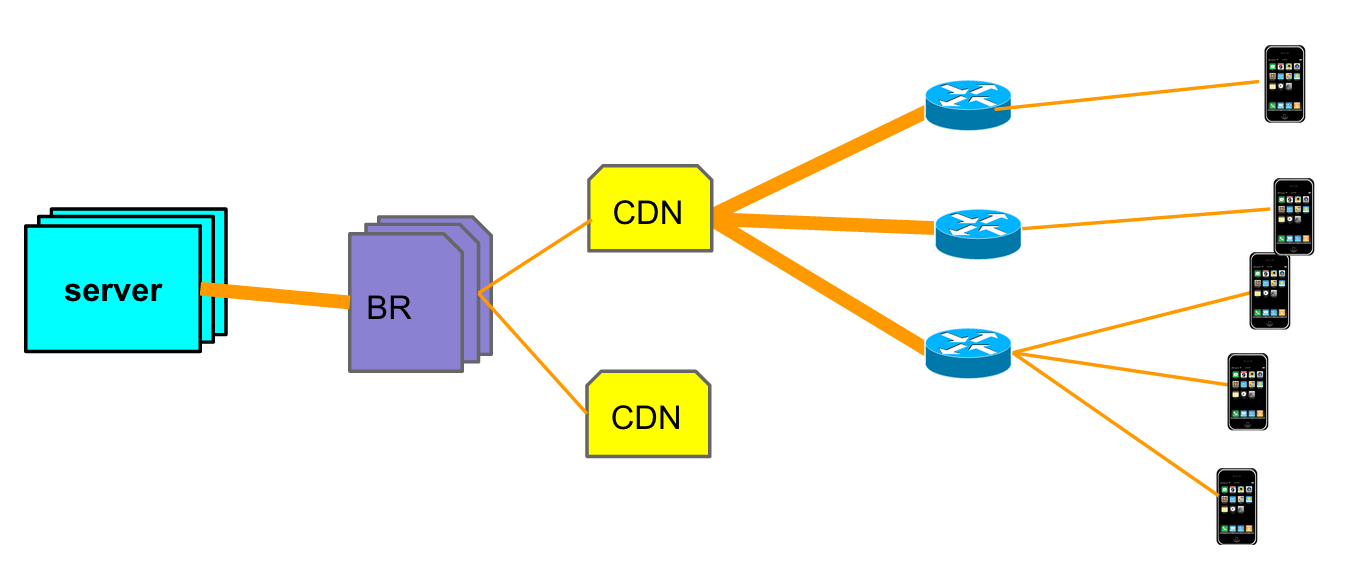
\includegraphics[scale=0.3]{pic/central_archi.png}
\end{center}
\caption{centralized video system architecture}
\end{figure}

However, current video systems are not optimized for the ever increasing bandwidth consumption. Current video streaming systems mostly use the centralized architecture as shown in Figure 2. In this architecture, the same copy of data will be transmitted over WAN for multiple times even when two clients are very close to each other. WAN bandwidth is not properly utilized. Besides, the central server or a CDN server may be overwhelmed by a large demand. 

The problems existing in the centralized server lead us to think if we can build a decentralized video system. And we do find two good opportunities. The first one is that bandwidth is very large now for both wired LAN and wireless LAN. Wired LAN is known to be very fast for a long time. For wireless LAN, the recently approved 802.11 ac protocol has a maximum bandwidth of about 1300 Mbps, which is a significant improvement from its predecessors. Large available LAN bandwidth means that we do not need to worry about the last hop communication. All we need to care about is how to effectively transmit video streams from the source to the local access point. The other opportunity comes from cloudlets~\cite{simoens2013scalable}. Cloudlet is attached to the local access point (AP) and has reasonable computation power. Because it's attached to AP, all the clients can communicate with the cloudlets via LAN. With its computation power, we can dynamically do adaptations to better serve videos based on the current network conditions. These two features make cloudlet the best fit to build an application layer multicast system.

In this paper, we propose a new decentralized video streaming system. In our system, there is no central streaming server. All the cloudlets are connected with cloudlets via LAN. All the cloudlets are connected with other cloudlets via WAN. We have a central metadata server to manage the overlay tree structure of the cloudlets. Only control data are transmitted between cloudlets and metadata server so that it will not have a bandwidth bottleneck in the metadata server. By doing ALM, we effectively reduces bandwidth consumption from linear to client number to linear to cloudlet number. Because of the ample LAN bandwidth and reasonable computation power on cloudlets, one cloudlet can server tens of cloudlets. Thus, our system can reduce bandwidth consumption by an order of magnitude in the best situation. This paper makes the following contributions:

\begin{itemize}
  \item It describes the benefits of a live streaming system on the new wearable devices, identifies the technical challenges in scaling such a system, and analyzed why the current architecture cannot satisfy a huge demand in the future.
  \item It proposes a new decentralized architecture to do Internet scale live streaming broadcast. This architecture is built on top of cloudlets and achieves scalability by using ALM to reduce bandwidth consumption on WAN and solve the single point bottleneck. It describes the tradeoffs in the design process.
  \item It builds a running system on cloudlets and Google AppEngine. It includes the server codes on cloudlet, metadata code on Google AppEngine and client code on Google Glass. The client code is used just used for a demo. As we make no assumptions on clients, developers can easily build their own client and use our service. This whole project is open sourced to all that are interested in this work.
  \item It evaluates the system on its scalability, bandwidth efficiency, video quality and fault tolerance.  
\end{itemize}

Section 2 describes the overall architecture of our decentralized live streaming system. Section 3 describes the design of the cloudlet server which are effectively streaming servers on cloudlets. Section 4 describes the design and implementation of the metadata server which manages the overlay tree structure. Section 5 describes the fault tolerance mechanism of the system and tradeoffs in the design space. Section 6 has performance measurements of the implemented system on different configurations. Section 7 discusses related work. Section 8 discusses future work. Section 9 is the acknowledgment. Section 10 describes where and how to get the source code of the system.

\section{System Architecture}

\subsection{System Goals}
Our goal is to build a scalable live streaming system. To be more specific, it has two major goals:

\begin{enumerate}
  \item Our system should be scalable for stream uploading
  \item Our system should be scalable for stream downloading
\end{enumerate}

We specifically split stream downloading and uploading because most of the current systems and researches only focus on stream downloading. And we believe, with more and more wearable devices which could conveniently upload streams, stream uploading would be a bottleneck as well.

Except for those two major goals, we also have two additional bonus goals:
\begin{enumerate}
  \item A smaller latency would be better
  \item A smaller control traffic is better
\end{enumerate}

Smaller latency is better but we do not require that the latency should be very small. Our live streaming system is not meant to be an interactive system. So when we need to make a tradeoff between latency and bandwidth, we would pick bandwidth. 

The same goes to control data. Smaller control data would reduce the response time and save bandwidth. However, control data is quite smaller compared with streaming data. So we would not emphasize on control data. 

Besides, the system requirements, we also have some features to use to build the system. Taking advantage of these features makes our system much easier to design and better serve the requirements. The good thing is that we are building a live streaming system. Live streaming could give us the below benefits in building our system.

\begin{enumerate}
  \item Data is live streamed. There is no need to store data.
  \item All the clients are actually requesting the same data. Unlike on-demand videos, people may be viewing the same video at different time. For live streaming, people are always watching the current time.
\end{enumerate}

No data needs to be stored. This gives us the opportunity to build a fully distributed system. We do not need a central server to store the data. Central server would always be a bottleneck and without it we could build a fully distributed scalable live streaming system.

All clients are requesting the same data. So we do not need to get different data from different clients in the peer-to-peer scheme. We could randomly pick a peer and that data must be the data this client is requesting. This makes our scheme much easier.

\subsection{Overlay Forest}

Our system is an Internet scale decentralized video steaming system. As shown in Figure 3, we build an overlay forest on top of the WAN. The nodes in the forest are cloudlets. The green line means WAN stream data. The blue line represents LAN stream data and the dotted line is WAN communication data. So we can see that cloudlets connect with other cloudlets via WAN. The root of a single tree (blue nodes in the forest) is the cloudlet that acts as the stream sender. The forest and tree structure is managed by a metadata server. All the clients communicate with cloudlets via LAN. This is not part of our overlay forest because our system only cares about WAN communications. 

\begin{figure}[t]
\begin{center}
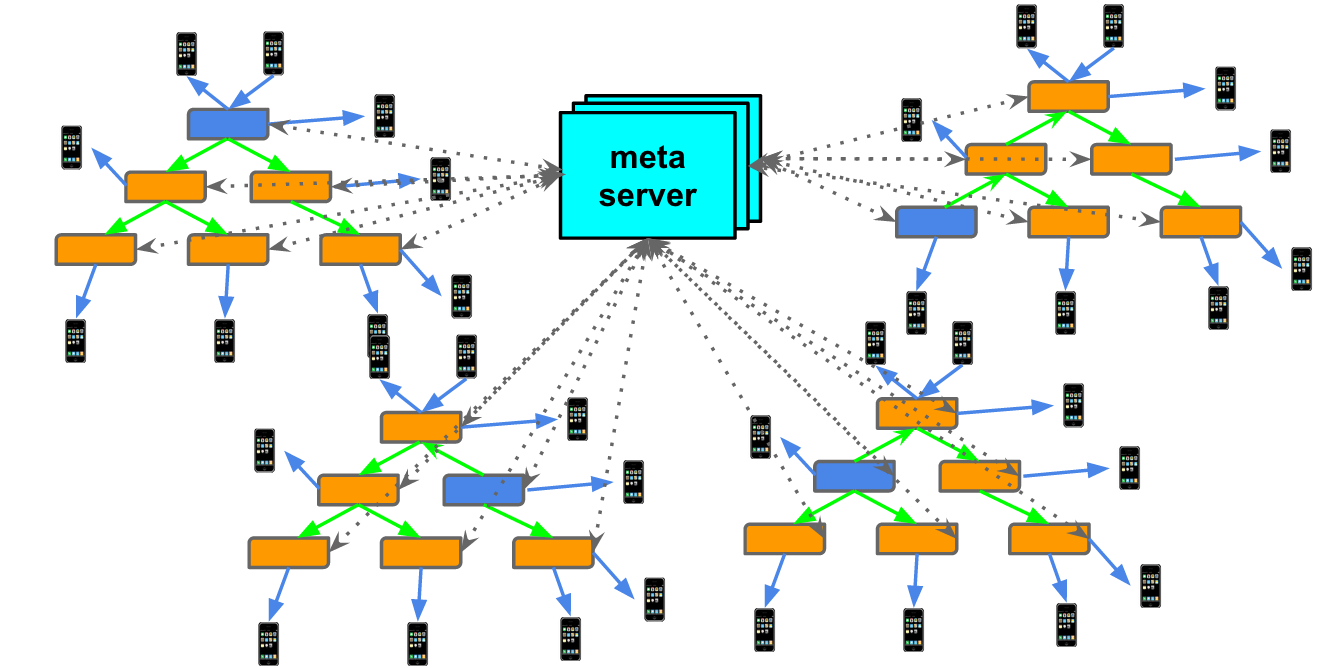
\includegraphics[scale=0.3]{pic/overlay_forest.png}
\end{center}
\caption{system architecture}
\end{figure}

\begin{figure}[h]
\begin{center}
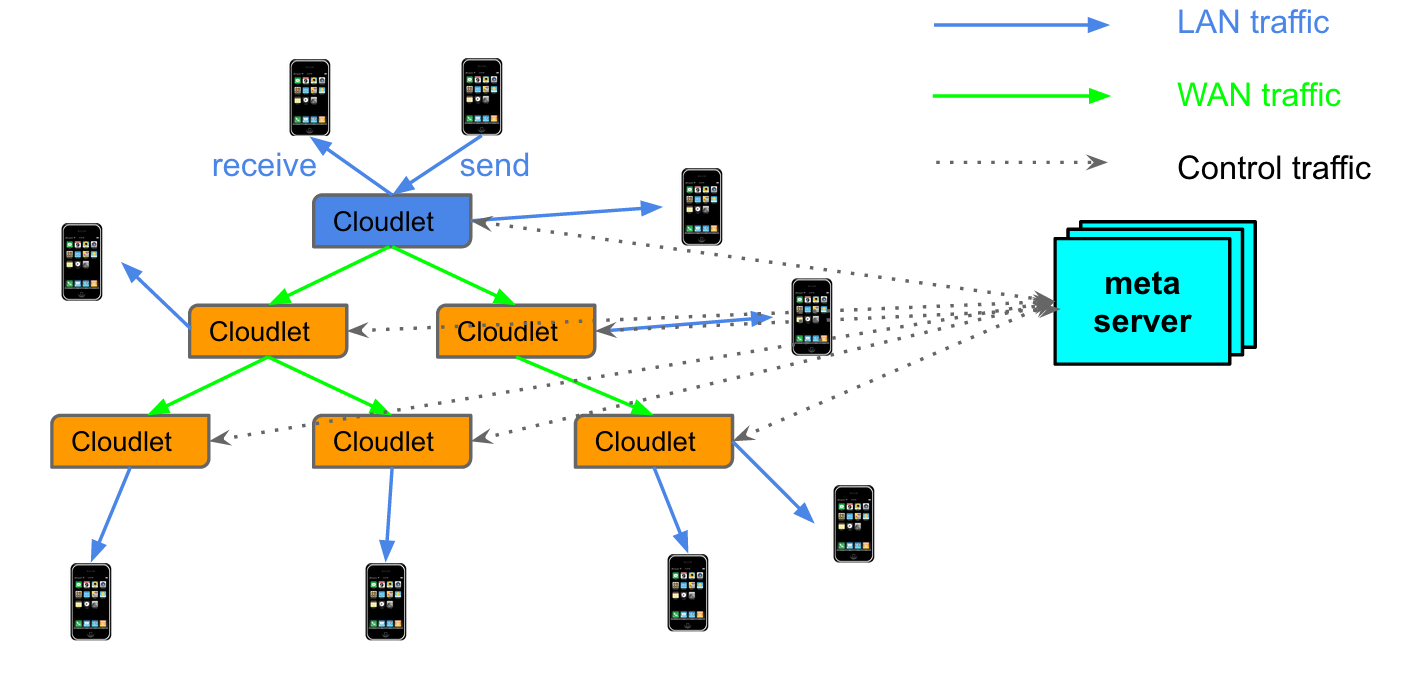
\includegraphics[scale=0.3]{pic/overlay_tree.png}
\end{center}
\caption{overlay tree structure}
\end{figure}

One tree represents one specific stream with one sender and multiple receivers. Our system supports multiple streams with multiple receivers. For each specific stream, the structure and operation are similar. Figure 4 shows one stream in the forest. Each cloudlet could have heterogeneous computation power and bandwidth capacities. They will report their current machine status and stream status to the metadata server repeatedly via a heartbeat message and the metadata server will then decide the tree architecture accordingly. 

\begin{figure}[t]
\begin{center}
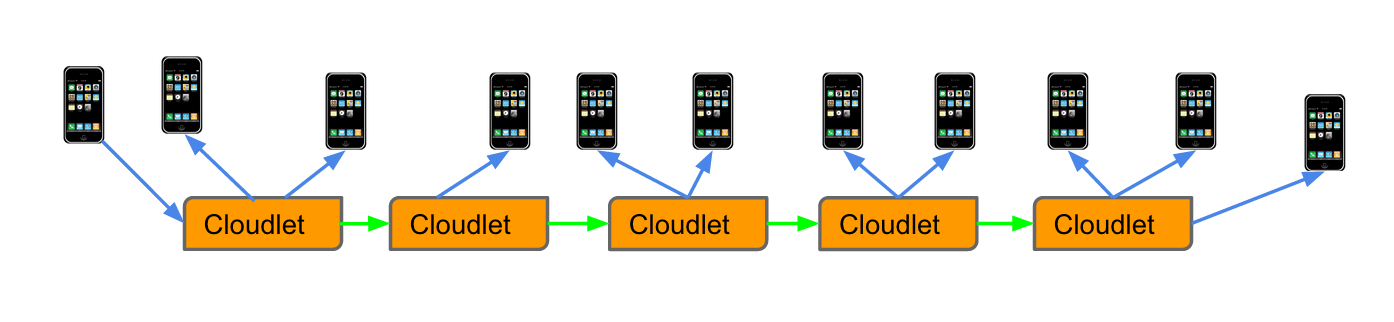
\includegraphics[scale=0.3]{pic/line_structure.png}
\end{center}
\caption{line structured overlay tree}
\label{fig:line_structure}
\end{figure}

Tree structure affects the system performance a lot and each tree structure reconfiguration will take a reasonably long time. So each tree construction decision is made with caution by the metadata server. The tradeoff in the design space here in tree structure is mainly about latency and bandwidth consumption. If we line the cloudlets up in a straight line as shown in Figure~\ref{fig:line_structure}, we will have the smallest bandwidth consumption on WAN. Each cloudlet just needs to send out one copy of data on the WAN. However, the price we take here is the latency. The tail nodes have to wait for all the previous nodes doing buffering and sending it the data it needs. 

\begin{figure}[h]
\begin{center}
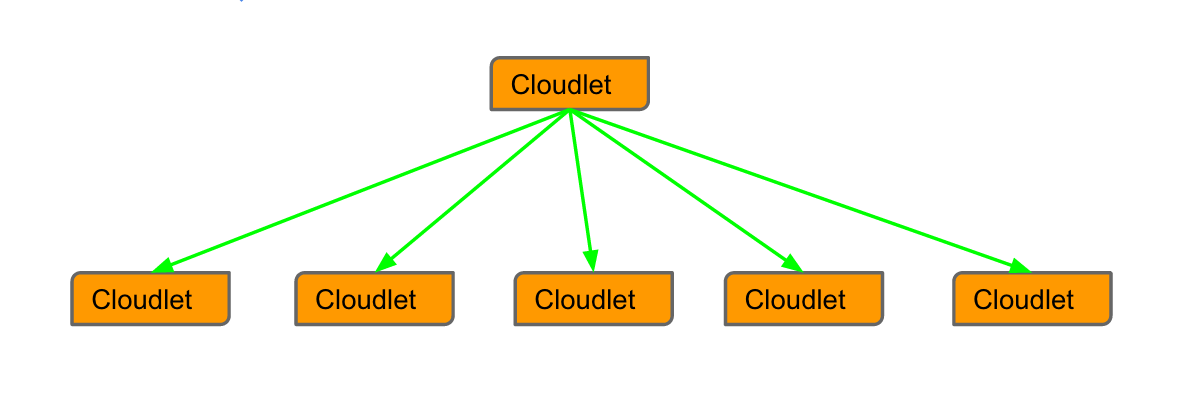
\includegraphics[scale=0.3]{pic/large_fanout.png}
\end{center}
\caption{large fanout structured overlay tree}
\label{fig:large_fanout}
\end{figure}

If we use a structure with large fanout at each node as shown in Figure~\ref{fig:large_fanout}, our decentralized model will degrade to a centralized model when the fanout is big. The same problems with the centralized architecture will come back, although we enjoy a smaller latency here.



\subsection{System Design Assumptions}

Our system makes certain assumptions about the environment our system will be used. They affect our design choices in later sections. The assumptions are:

\begin{enumerate}
  \item LAN always has ample bandwidth. WAN does not.
  \item Bandwidth is important. Latency is not as important.
  \item Clients are not reliable.
  \item Cloudlet can fail. Network could be partitioned but these kind of failures will not occur frequently.
\end{enumerate}

For assumption 1, we have proved that using the current technology parameters. This is the reason why we build our system. For assumption 2, we are building a live streaming broadcasting system, not a video chat system. Latency is not the key factor we are considering now. When there are conflicts between latency and bandwidth, we will favor bandwidth. Of course, high latency is not what we want. So we will reduce the latency to the best as long as bandwidth is not sacrificed. For assumption 3, we expect that more and more clients will be mobile and wearable devices that are connected to the Internet via wifi. They are not reliable. They may lose connection at any time. For assumption 4, cloudlet is not like clients. They are servers in a safe box and connected to the Internet with wires. They are less reliable than servers in data centers but are high more reliable than clients.

\section{Cloudlet Server}
\label{sec:cloudletServer}

\subsection{Server Design}
Cloudlet server is an abstraction of the service provider on cloudlets. It consists of three major components: streaming server, control server and a stream monitor. Streaming server is just an ordinary streaming server. It collects streams from senders and receivers can then get stream data from the stream server. Control server is the core of the cloudlet server. It receives requests from clients, asks streaming server to open or close a stream and communicates with the metadata server to update stream status. All the control data go to the control server. Stream monitor is a cron job that runs on the cloudlet. It's a bridge between the streaming server and the control server. Control server will get stream status information from the stream monitor rather than the streaming server. This additional layer of indirection makes control server and streaming server independent of each other. It adds flexibility and modularity to our system.

The cloudlet server opens 4 APIs for the clients:

\begin{itemize}
  \item openStream(userName, appName, streamName, streamBandwidth)
  \item closeStream(userName, appName, streamName)
  \item joinStream(userName, appName, streamName)
  \item exitStream(userName, appName, streamName)
\end{itemize}

We first expain the parameters in the APIs. Parameter \emph{userName} is used to identify the user requesting to send or receive a specific stream. It is used to do permission control. Some streams may be private to some particular users. Parameter \emph{appName} and \emph{streamName} is used to identify a specific stream. There can't be two streams with the same appName and streamName. We added the \emph{appName} to make our system more general to support multiple applications. Parameter \emph{streamBandwidth} in the openStream API is used for an estimation of the uploading video. This quality is estimated by clients and sent to the server. Our server may update this value when it finds the real stream bandwidth consumption is different to the estimated value to a big extent.

\emph{openStream} is used for a client to start broadcasting live streaming data. \emph{closeStream} is used for the stream broadcaster to stop serving data. If the client forgot to do that, that's fine. Our system will detect it and call this API. \emph{joinStream} is used by a client to receive a specific stream. \emph{exitStream} is used by a client to exit receiving the stream. Also, it the client forgot to call this API, we will detect it and call it for the client. 

\subsection{Streaming Server}
Our streaming server uses Nginx with rtmp module. Nginx is an open source server. With rtmp module, it can receive and provide stream data in rtmp protocol. rtmp protocol is widely used in live streaming serving and is also what our system accepts. Nginx with rtmp module supports multiple application and multiple streams. It satisfies our need to be a general live streaming service provider. 

To build a streaming system is hard and needs much knowledge on streaming codec and resource management. That's why we choose to use Nginx with rtmp module. It greatly reduces our development efforts in building the system. However, it do come with some problems. The first one is for buffering. Nginx with rtmp module will require a buffering to recognize the codec of the incoming stream. This is the main source of latency. Secondly, it do provide APIs to get the streaming status in the streaming server. However, to reduce resource consumption, it does so with a fixed length of time. This time is not configurable. This makes our detection of failures take a longer time.

To fully control the incoming stream and connect cloudlets, we use ffmpeg~\cite{tomar2006converting} to create a stream pipe connecting two streaming servers. Ffmpeg is widely used in all kinds of video processing and transmitting jobs. It's open sourced and supports all the common video and audio codec. The price comes with this design is also the latency because ffmpeg will do buffering as well.

\subsection{Control Server}
The control server is a http server built with Django. All the control messages from clients and the metadata server will go to this server. The APIs open to the clients are all implemented in the control server.

When a client wants to broadcast live streaming video, it will call the \emph{openStream} API of the control server. Then the server will first check if this user can broadcast the video with the user defined application name and stream name. If it can , the control server will communicate with the metadata server and become a root node of the stream overlay tree in the metadata server. Then the server will tell the client to transmit video data to the stream server and this stream is marked available in the control server.

When a client wants to exit broadcasting live streaming data, it will call the \emph{closeStream} API. Then the control server will tell the metadata server to destroy the stream tree it previously built. Then it tells the streaming server to stop receiving and offering data of this stream and mark this stream as finished in its internal data structure.

When a client wants to watch a stream, it tells the control server by calling the \emph{joinStream} API. Then the control server will first check if it already has this stream available. If so, it direct the client go to the streaming data directly for the stream it wants. If not, it will go to the metadata server to ask for the name of a cloudlet holding the stream data. After getting the cloudlet name, it will create a pipe between the streaming servers on the two cloudlets by using ffmpeg. Then it directs the client to the local streaming server for the stream data.

When a client wants to exit watching a stream, it tells the control server by calling the \emph{exitStream} API. Then the control server will check if there are other clients in the same LAN watching the stream. If so, it does nothing. If not, it tells the metadata server to delete itself from the stream tree and mark the stream in its internal data structure as finished.

The control server also needs to send heartbeat messages to the metadata server to repeatedly report the machine status and the stream status. For machine status, it includes current bandwidth consumption and packet loss rate. Streaming server is IO intensive, so we do not send CPU usage or memory usage to the metadata server. Stream status includes bandwidth usage on each stream, number of cloudlets connecting to this cloudlet for the stream and number of clients connected to this cloudlet for this stream.

The control server acts both as client and server. For the real clients, it is a http server. For the metadata server, it acts as a client and send http request to the metadata server. In all of our client-server communications, we use pull strategy. Only client will send requests to the server. The server will never initiate a request to the clients. This simplifies our system design and makes the fault tolerance easier. We will talk more about that in section 5.

\subsection{Stream Monitor}

The stream monitor is a cron job running on the cloudlet. It is a middle layer between the streaming server and the control server. It repeatedly collects stream information from the streaming server by analyzing the statistic file the Nginx server generates and updates. It has two communication channels to the control server. When everything is normal, the stream monitor repeatedly report stream status to control server in a fixed time interval. If it detects anything irregular, it will directly report error to the control server and the control server will decides further actions. This part will be discussed more in section 5 fault tolerance. 

Stream monitors in the system is critically important. It acts as sensors. There may be inconsistency between cloudlet control server and metadata server, and/or inconsistency between control server internal data structure and the real situations. All the final decisions are made based on the information provided by the stream monitor. When any inconsistency is found between the metadata and the information provided by the monitor, the monitor wins and the internal data structure will be corrected.


\section{Metadata Server}

\subsection{Server Design and Implementation}
Metadata server is the most important part in the whole system. It constructs, expands and maintains the overlay tree structure. In case of failures, it's responsible for reconstructing the overlay tree structure. Therefore, we want to make this server extremely available. Besides, all the cloudlets will send heartbeat and other requests to the metadata server. It will not consume large bandwidth but it do impose a the problem of single point failure. So we decided to build this server on Google AppEngine. Google's cloud infrastructure will offer us scalability and reliability. All the servers are stateless. They receive http requests and return http responses. The states of the system is safely stored in the datastore all servers share. Datastore is built on BigTable by Google and has great availability and scalability.

Metadata server opens APIs for cloudlet control servers. Only the control server will call those APIs. They are completely hidden to clients. Those APIs are:

\begin{itemize}
  \item initNode(cloudletName, maxBandwidth)
  \item createTree(cloudletName, appName, streamName, streamBandwidth)
  \item exitTree(appName, streamName)
  \item joinTree(cloudletName, appName, streamName)
  \item heartbeat(cloudletName, cloudletStatus, streamStatus)
\end{itemize}

\emph{initNode} will be called when the cloudlet starts service. It will only be called once. When the metadata server receives this request, it will create a cloudlet data structure to represent the cloudlet which initiates the request. An important parameter of this API is the \emph{streamBandwidth}. It's the maximum bandwidth the cloudlet thinks it has and the metadata server will not break this whenever it has another option.

The control server will call \emph{createTree} when a client requests broadcasting a stream. Metadata server will create an overlay tree rooted on the requesting cloudlet after receive this request.

The control server will make \emph{exitTree} request when the sending client finishes serving data or all the viewers in the same LAN with the cloudlet exited watching. Metadata server will first check the position of the requesting cloudlet in the overlay tree. If it's the root node, it destroys the whole tree. If it's from a non-root cloudlet, it will check whether it's a leaf cloudlet. A leaf cloudlet means that no other cloudlets depend on this cloudlet to get data of this particular stream. If it is a leaf cloudlet, it is safe to exit. If it is not, the metadata will not allow it to exit because once it stops serving the stream data, all its descendents in the subtree rooted on this cloudlet will need to be reconfigured to other cloudlets. This will stop the stream on those cloudlets for about 30 seconds. The metadata server will instead make that cloudlet as a dummy node in the overlay tree structure. The new coming cloudlets will not be scheduled to a dummy node. So the intermediate descendents of that node will never increase. We will exit that node when it becomes a leaf node. 

When a cloudlet has a request from clients asking for a stream it does not have now, it will make a \emph{joinTree} request to the metadata server. The metadata server will respond with the cloudlet name of a cloudlet serving that stream. That cloudlet is chosen by a scheduling algorithm. That algorithm will be described in the next subsection. 

Control server sends \emph{heartbeat} messages to the metadata server with its own status and stream status. This keeps the cloudlet alive in the metadata server. Whenever a cloudlet has not contacted the metadata server for a pre-defined time interval, it will mark this cloudlet as unavailable. New cloudlets will not be scheduled to an unavailable cloudlet. The metadata server will not delete the node representing that cloudlet in the overlay trees because this can best keep the subtree structure. 

\subsection{Scheduling}
Scheduling algorithm determines the overlay tree structure. The tree structure will then affect bandwidth consumption on WAN and latency. Our scheduling algorithm will favor bandwidth to latency as we explained in section 2. The general idea of this algorithm is to search from the root using breadth first search (BFS) to find the first node with enough available bandwidth for serving this stream. We use BFS because we want to find a cloudlet nearest to the root so that it has the smallest latency. In the cases of inconsistency and failures, the algorithm may find the cloudlet requesting to join tree has already been in the tree. In this case, we delete the old node and re-schedule the node to another node in the overlay tree that is not in the subtree rooted on that cloudlet in the old tree configuration. If the algorithm finds that no available nodes are there, it will randomly pick one node to serve the data. The algorithm is shown in the code snippet below. 

{\tt \small
\begin{verbatim}
Cloudlet schedule(Cloudlet cloudlet,
              overlayTree tree) {
    TreeNode node = tree.find(cloudlet);
    Cloudlet ret = null;
    if (node != null) {
        ret = bfs(tree);
        if(ret == null){
            ret = randomPick(tree);
        }
    } 
    else {
        delete node from tree;
        ret = schedule(cloudlet, tree);
    }
    return ret;
}

Cloudlet bfs(overlayTree tree) {
    int streamBand = tree.getBand();
    TreeNode node = tree.getRoot();
    while(node != null) {
        if (node.leftBand > streamBand) {
            return node.getCloudlet();
        }
        node = tree.getNextBfsNode();
    } 
    return null;
}

\end{verbatim}
}

\section{Fault Tolerance}

\subsection{Fault Sources}
Our system is intended to be an Internet scale live streaming system. In a large scale, all the components may fail and we must be able to tolerate all those failures. Here we identify the possible failures in different components and explain the possible effects of those failures to our system.

\paragraph{client}
Clients failures are normal, especially when clients are mobile or wearable devices. Network connection between those clients and the servers can easily break because a small movement in space. Besides, Users will usually not follow the best practice of using an application. It's very likely that they will just force the application the exit rather than gracefully exit it. Client devices also have a higher possibility to fail, OS breakdown and machine failures are all possible. To our system, client failures are considered normal and will not break our system, no matter the client is a sender or a receiver. Our system will detect those failures and clear inconsistent internal data structure and resources.

\paragraph{cloudlet}
Cloudlet failures are also possible. Possible causes are power failures, network partition, OS failures and hardware failures, etc. However, the possibility of cloudlet failures are much lower than the client failures because they are well protected machines in a box. If the cloudlet server is down, the clients in the same LAN with the cloudlet cannot use our service till the cloudlet is back again. However, for clients in other LANs, our system guarantees that the fault will be fixed and their service will be back as long as the sender is working. Our fault tolerance protocol will mainly tolerate failures caused by cloudlets failures.

\paragraph{metadata server}
Metadata server failures are very unlikely because we built the server on Google AppEngine and used the high replicated datastore that will distribute data to different data centers. Google AppEngine will provide high availability to our system. However, in the extremely rare cases of Google's failure, our system is down. No more clients can send or receive streams. Only the currently working ones can use the old setting to continue use the service till they exit or other failures occurs.

\subsection{Fault Tolerance Protocol}
All the cloudlet servers are distributed across the Internet. Every node may fail. We have a general distributed protocol to guide all the cloudlets to communicate with each other and make a system wise good decision in case of failures. This protocol includes three major parts, failure detection, failure source identification and failure correction.

\paragraph{failure detection}
Failure detection is the first step in fault tolerance. To tolerate a fault, a cloudlet must first detect it. Our system uses stream monitor to detect a failure. Stream monitor on each cloudlet will monitor the incoming bandwidth for each stream. If the incoming bandwidth of a stream is zero, it means there must be some failures in this stream. It might be network partition or machine failures. The root cause of the failure does not matter for that cloudlet to restore service. The effect of any kind of failure will cause incoming stream bandwidth to be zero. We only deal with faults when a failure has caused some real effects on some cloudlets. There might be inconsistencies in the cloudlet server's internal data structure and the metadata server's data structure. Those inconsistencies are most likely to be caused by failures. But we do not consider them as failures because it's very hard to know which failure on which machine caused the inconsistency.

\paragraph{failure source identification}
When on cloudlet failed, all the other cloudlets in the subtree rooted on that cloudlet will not get streaming data of that stream. However, we do not want all the cloudlets to start their restoration independently because this will cause a network reconfiguration chaos. The network structure will change a lot. Our approach is when a cloudlet detected failures on a stream, it will first identify the source of the failure. For a specific cloudlet, there are just two kinds of failure sources, its previous node failed or some nodes in prior to its previous node failed. To identify this, it will simply pass a inquiry to its previous node asking the status of that stream in the previous stream. If the previous node responded and the response is that it is also waiting for that stream, this cloudlet will know its previous node is fine and nodes prior to that have failures. Otherwise, it will mart its previous node as failed.


\paragraph{failure correction}
After identify the source of failure, the cloudlet will correct the failure. If the immediate previous node of this cloudlet is failed, this cloudlet will send a message to the metadata server asking for a re-scheduling and then create a pipe to that new node and clear the resources occupied by the old pipe. If the immediate previous node of this cloudlet is not the source of failure, it will do nothing and just believe that the immediate descendents of the failed node will fix the problem.

\begin{figure}[t]
\begin{center}
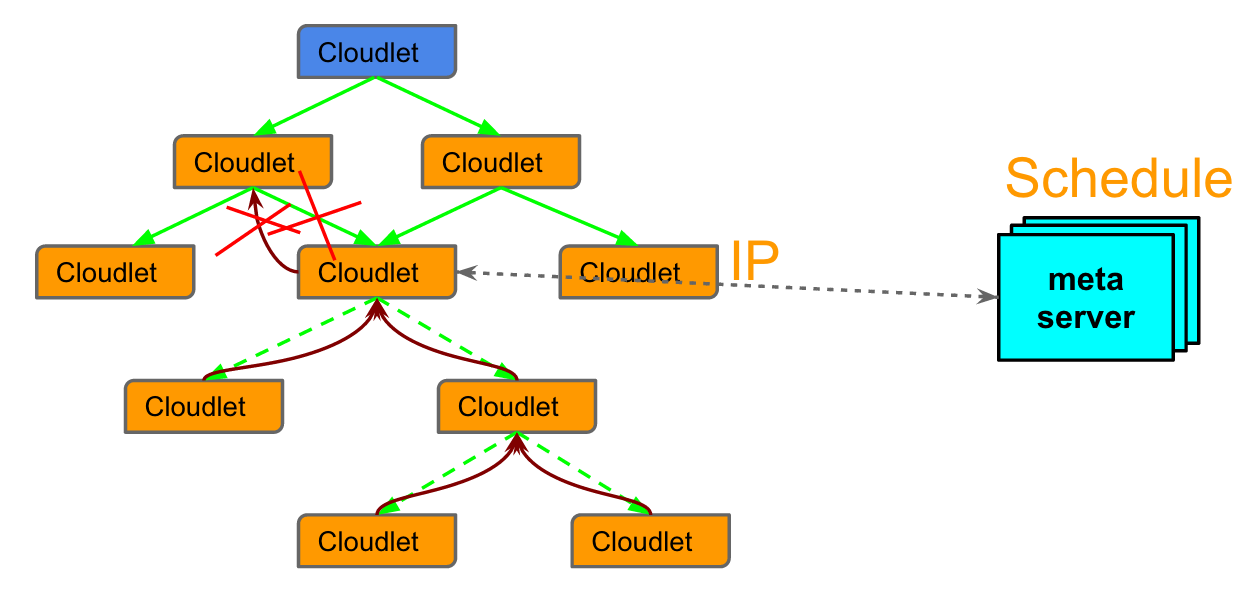
\includegraphics[scale=0.3]{pic/fault_tolerance.png}
\end{center}
\caption{line structured overlay tree}
\label{fig:fault_tolerance}
\end{figure}

The whole fault tolerance protocol is illustrated in Figure~\ref{fig:fault_tolerance}. The dotted green line means the network is working but no stream data is on that line. The brown line is the inquiry message to the previous node. Before each cloudlet that detected a failure to reschedule to another node. They will first identify the source of failures and based on its relative to the position of the failed node they will make different decisions. This approach can best keep the current tree structure and reduce control data.

\section{Experiments}
\subsection{Evaluation Objective}
By doing the experiments, we want to prove that our system is effective. To be effective, our system needs to satisfy the following two requirements:

\begin{enumerate}
  \item It effectively reduce bandwidth consumption on WAN.
  \item It best keep video quality
\end{enumerate}

Reducing bandwidth consumption on WAN is the primary goal of building this system. We want to reduce both the overall bandwidth consumption on WAN and on individual cloudlet server. 

Best keep video quality means the video quality will not degrade in the transmitting process unless the network condition is to bad and we choose to degrade resolution in order to keep smoothness. To measure video quality, we use two parameters: bit rate in the receiving player and packet loss rate. If the player has almost the same bit rate as the sender, we think that the video quality is not degraded and a low packet loss rate represents that smoothness is good. By using these two parameters, we avoid the inaccuracy and troubles in human measurements.

\subsection{Test Setting}
\begin{table}[t]
\begin{tabular}{|l|l|l|}
\hline
Component       & Location                & \#Instances\\ \hline
Metadata Server & Google AppEngine        & 2               \\ \hline
Cloudlet Server & OpenStack Cluster & 6               \\ \hline
Sender Clients  & Amazon Web Service      & 6               \\ \hline
Receive Clients & OpenStack Cluster & 10              \\ \hline
\end{tabular}
\caption{Cluster configuration}
\label{table:cluster}
\end{table}

\paragraph{Cluster Configuration}
To test our system, we used clusters on AWS, Google AppEngine and a local OpenStack cluster. The specific cluster configuration is listed in Table~\ref{table:cluster}.

\begin{table}[h]
\begin{tabular}{|l|l|}
\hline
Network Link & Link Bandwidth (Mbps) \\ \hline
Client -\textgreater Cloudlet & 746 \\ \hline
Cloudlet -\textgreater Cloudlet & 1.5 \\ \hline
Cloudlet -\textgreater Client & 932 \\ \hline
\end{tabular}
\caption{Network parameters}
\label{table:network}
\end{table}

\paragraph{Network Parameters}
To measure the performance of our system, network configuration and parameters are very important. In our experiments, we used WonderShaper~\cite{wondershaper} to do traffic control and the network parameter after shaping is listed in Table~\ref{table:network}.

\paragraph{Video Parameters}
To make testing process easy and repeatable and scalable, we choose to use a video clip and use the rtsp protocol, which is a widely used real time video transmitting protocol to upload it to the cloudlet server. This way, every time we do the experiment, data is the same and from the server's view it is just like a live streaming video. The video clip we choose is movie Sintel~\cite{sintel} from Durian open movie project. We used 640X480 resolution and the average bit rate under this resolution is 483 kbits/s.

\subsection{Single Stream Multiple Viewers Performance}

\begin{figure*}[t]
        \centering
        \begin{subfigure}[t]{0.3\textwidth}
                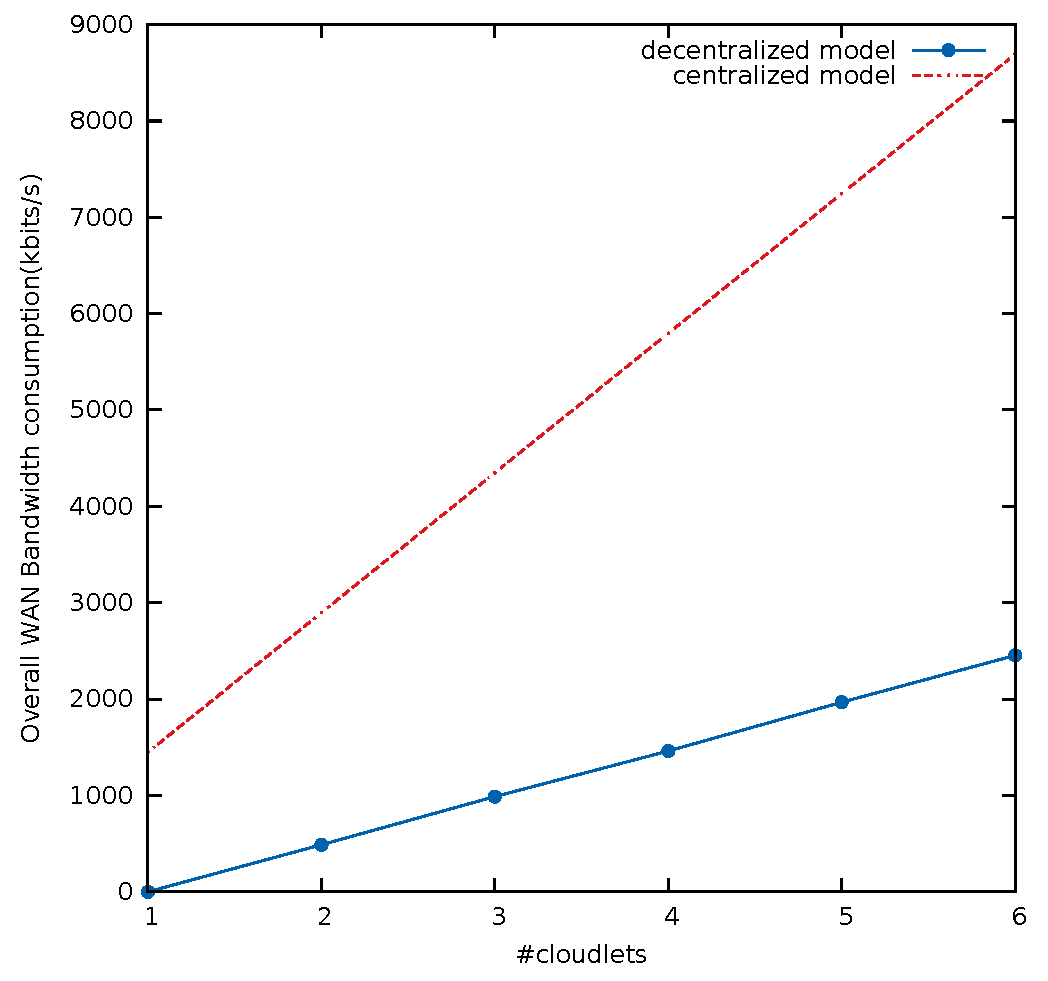
\includegraphics[width=\textwidth]{pic/overallBandwidth.eps}
                \caption{Overall bandwidth consumption on WAN}
                \label{fig:sinOverallBand}
        \end{subfigure}%
        ~ %add desired spacing between images, e. g. ~, \quad, \qquad, \hfill etc.
          %(or a blank line to force the subfigure onto a new line)
        \begin{subfigure}[t]{0.3\textwidth}
                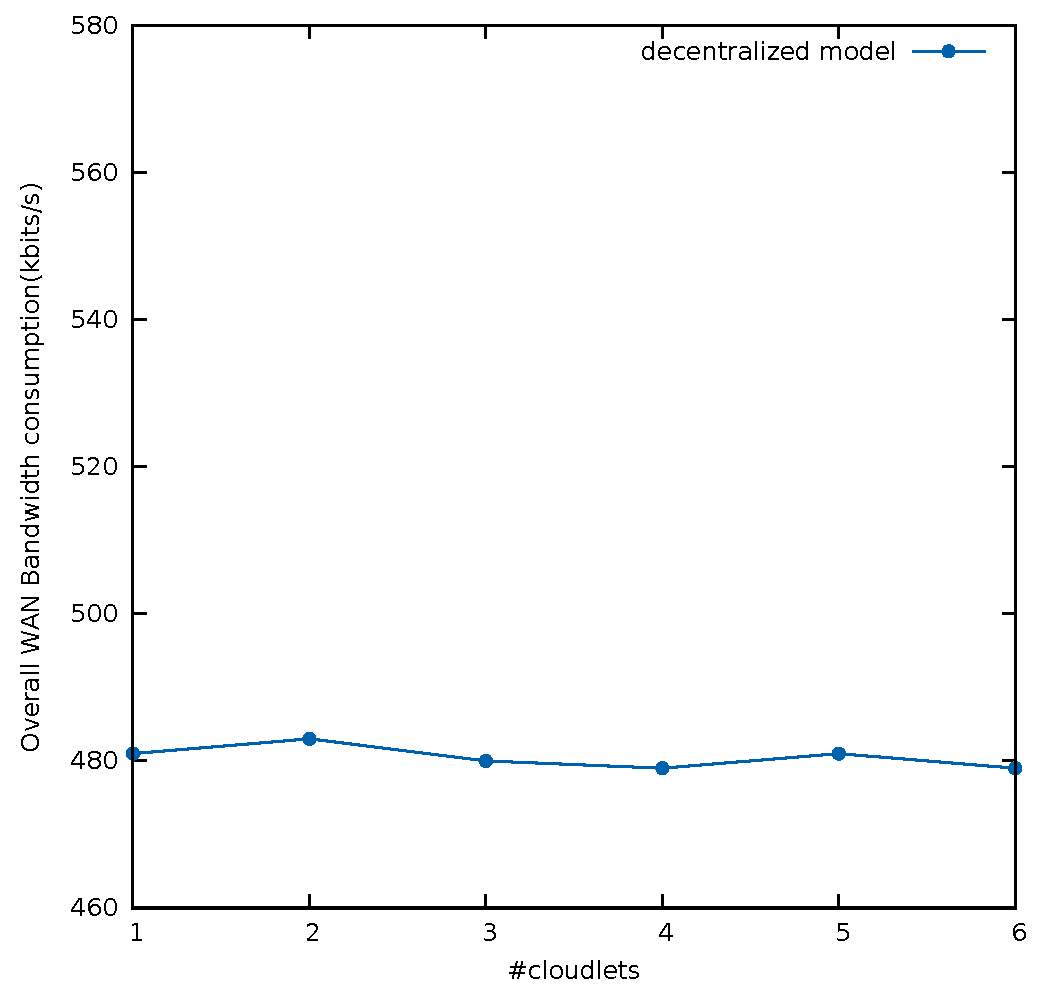
\includegraphics[width=\textwidth]{pic/perServerBandwidth.eps}
                \caption{Per server bandwidth consumption on WAN}
                \label{fig:sinPerServerBand}
        \end{subfigure}
        ~ %add desired spacing between images, e. g. ~, \quad, \qquad, \hfill etc.
          %(or a blank line to force the subfigure onto a new line)
        \begin{subfigure}[t]{0.3\textwidth}
                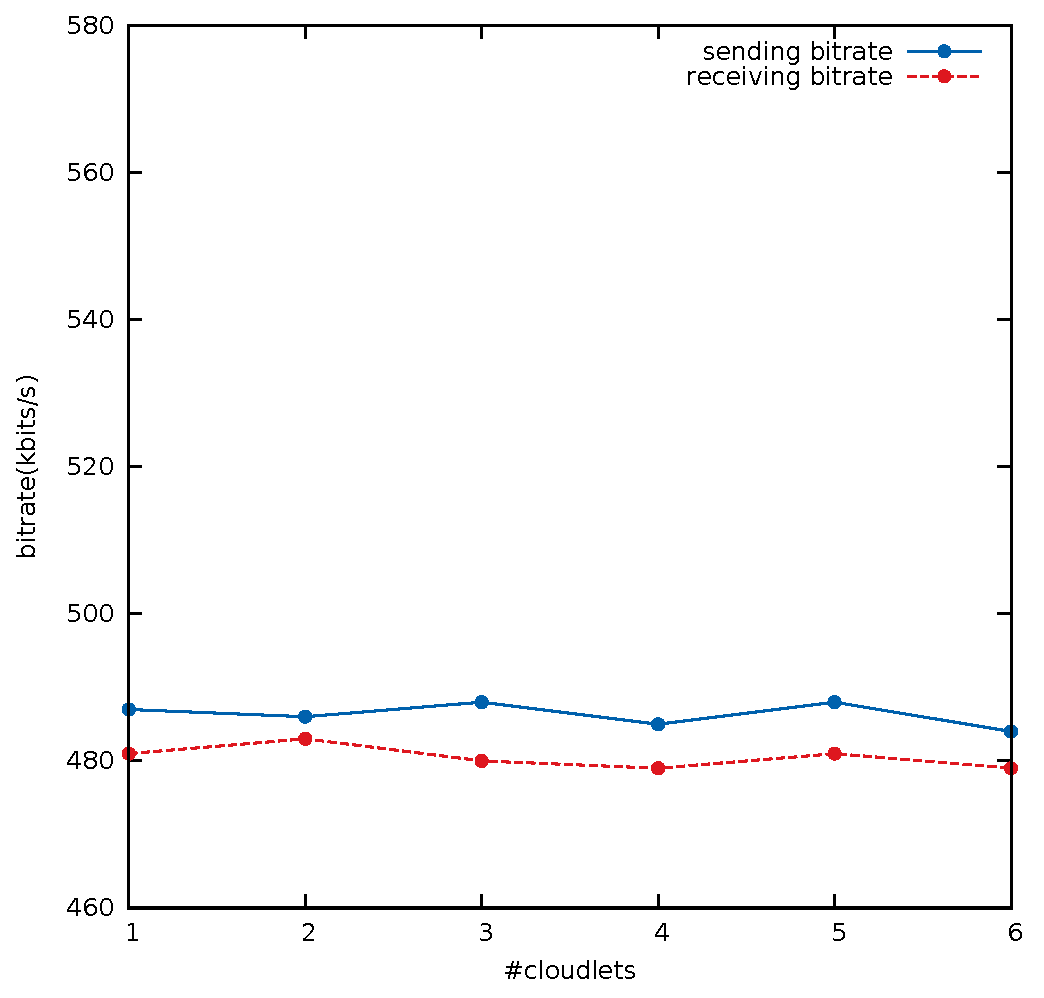
\includegraphics[width=\textwidth]{pic/sendingVsReceiving.eps}
                \caption{Sending and receiving bit rate comparison}
                \label{fig:sinBitRateComp}
        \end{subfigure}
        \begin{subfigure}[t]{0.3\textwidth}
                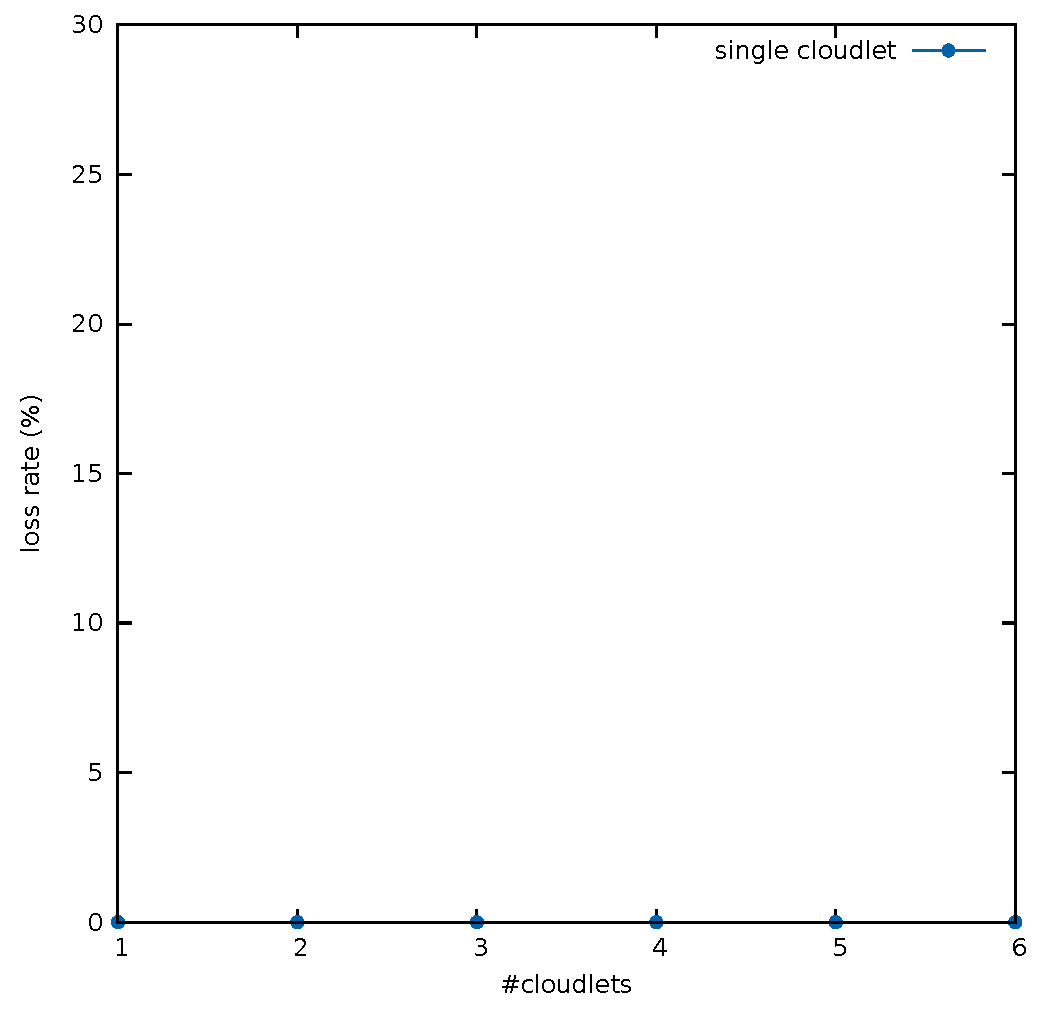
\includegraphics[width=\textwidth]{pic/lossrate.eps}
                \caption{loss rate of decentralized model}
                \label{fig:sinLossRate}
        \end{subfigure}
        \begin{subfigure}[t]{0.3\textwidth}
                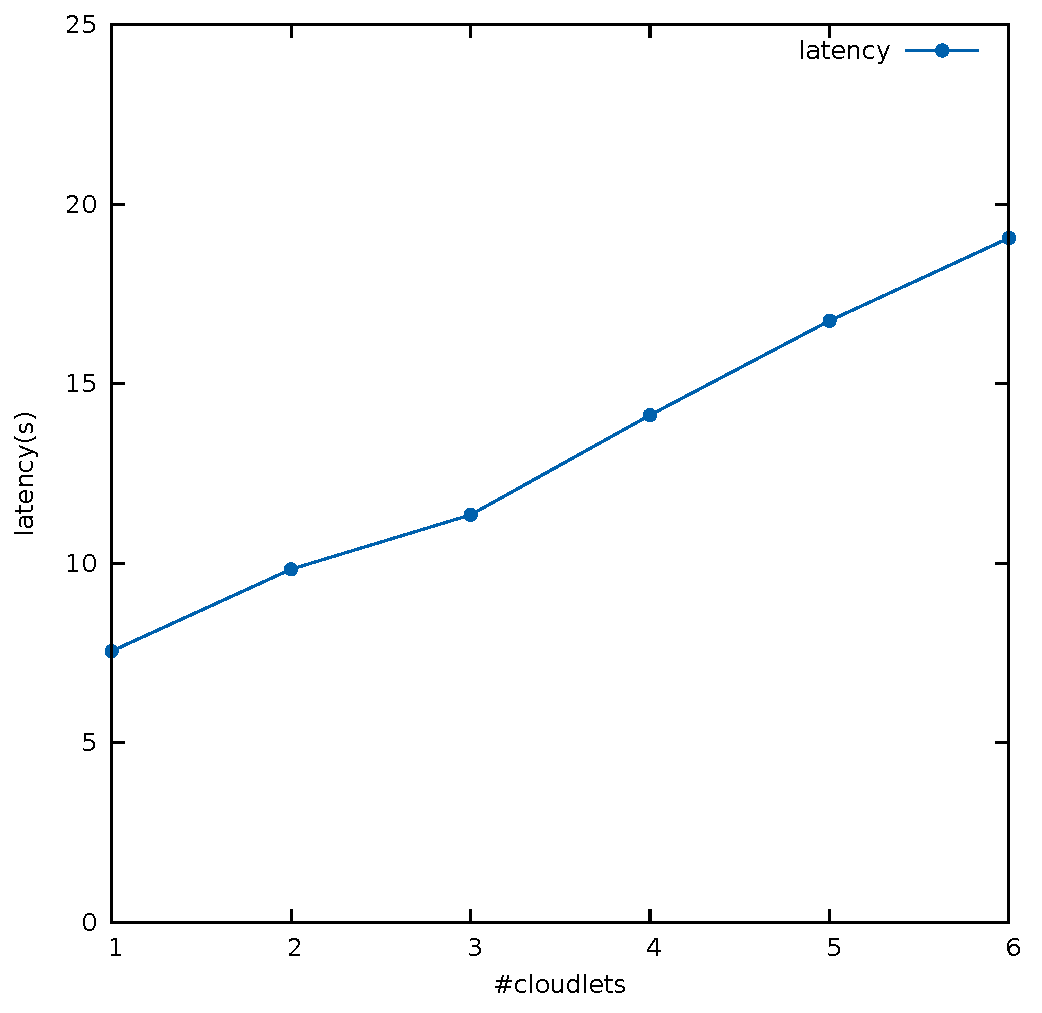
\includegraphics[width=\textwidth]{pic/latency.eps}
                \caption{latency of decentralized model}
                \label{fig:sinLatency}
        \end{subfigure}
        \caption{Experiment result for single stream multiple viewers case.}\label{fig:SingleStream}
\end{figure*}

Experiment results of the single stream multiple viewers use case is shown in Figure~\ref{fig:SingleStream}. Figure~\ref{fig:sinOverallBand} shows the comparison of the overall bandwidth consumption on the WAN under the assumption that each cloudlet will serve on average 3 clients. Since our decentralized model reduces the overall consumption from linear to number of clients to number of cloudlets, the overall WAN bandwidth consumption is one third that of the centralized model. 

The best part of our decentralized model is that is solves the single point bottleneck problem. When we line the cloudlets in a straight line structure, each cloudlet just needs to send out one copy of data to the WAN. Figure~\ref{fig:sinPerServerBand} shows the experiment results of this. Combining these two results, we conclude that our system can effectively save WAN bandwidth.

For video quality, we measured bit rate comparison of the sending cloudlet and the receiving player. The result is shown in Figure~\ref{fig:sinBitRateComp}. From that figure, we can see that the bit rate is almost the same. Senders will have slightly more traffic which is control data between the server and the client. Figure~\ref{fig:sinLossRate} shows the loss rate of our decentralized model. It's kept to zero. Combining bit rate and loss rate, we conclude that the video quality is not degraded in the transmission.

Those are the benefits brought by using the decentralized model. But it does come with a price, increased latency. Figure~\ref{fig:sinLatency} shows the latency with increasing cloudlet number. The relationship between the latency to the cloudlet number is almost linear. Each cloudlet will bring about 3 seconds more latency because of buffering.


\subsection{Multiple Streams Multiple Viewers Performance}

The multiple streams multiple viewers case is that many clients are sending streams to the same cloudlet and many clients from different cloudlets are watching this stream. This will impose another difficulty to our system. For the cloudlet with a lot of different uploaders, it is likely that those streams need more bandwidth than the cloudlet has. Because it is the source of all those streams, our decentralized model could not help relieve its burden. This may result in bad video quality for all those streams.

\begin{figure}[t]
        \centering
        \begin{subfigure}[t]{0.22\textwidth}
                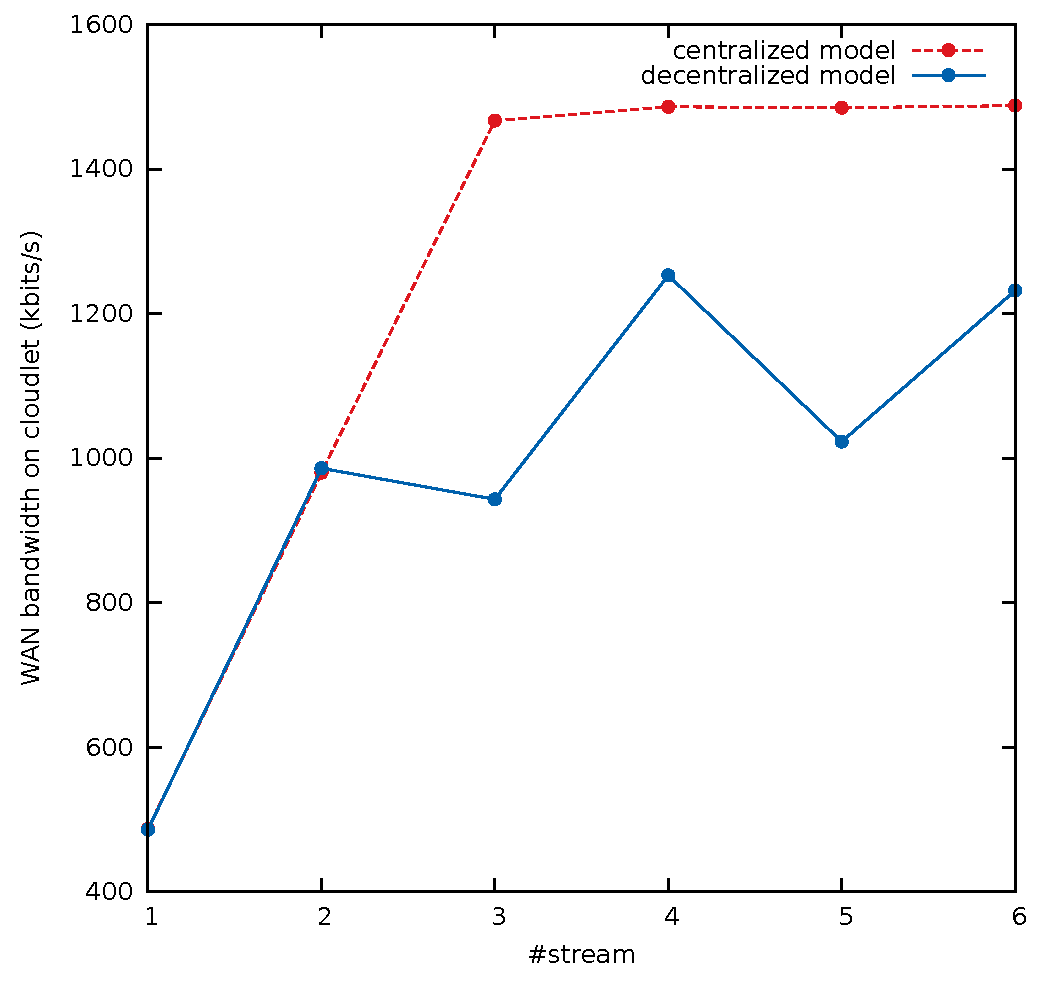
\includegraphics[width=\textwidth]{pic/multiBandwidth.eps}
                \caption{Bandwidth consumption on one cloudlet with multiple clients sending different streams}
                \label{fig:mulBandwidth}
        \end{subfigure}%
        ~ %add desired spacing between images, e. g. ~, \quad, \qquad, \hfill etc.
          %(or a blank line to force the subfigure onto a new line)
        \begin{subfigure}[t]{0.22\textwidth}
                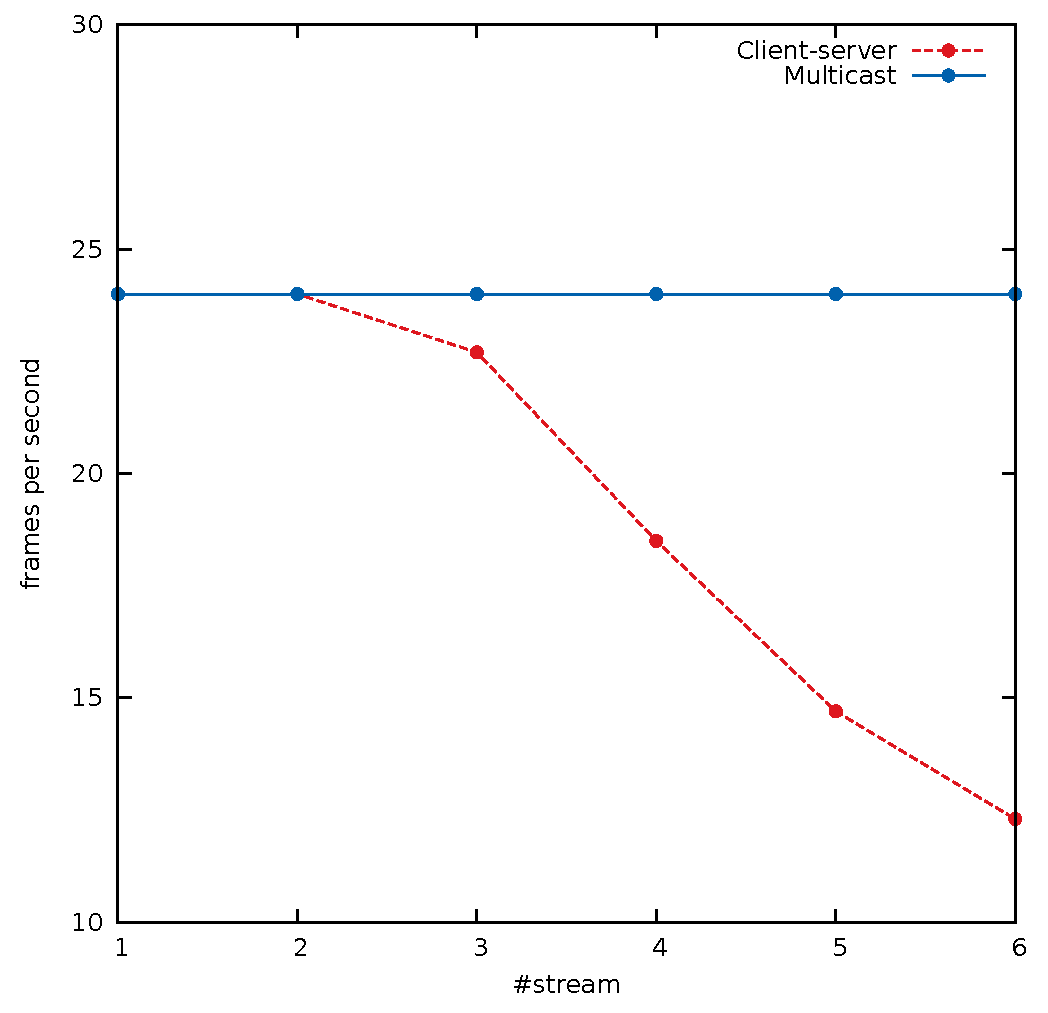
\includegraphics[width=\textwidth]{pic/fps.eps}
                \caption{Frame rate on receiving player of the requested streams}
                \label{fig:mulFps}
        \end{subfigure}
        \caption{Experiment results of multiple streams with multiple multiple viewers}\label{fig:MultiStream}
\end{figure}

What we did here is to degrade the video quality as described in Section~\ref{sec:cloudletServer}. As shown in the experiment results in Figure~\ref{fig:MultiStream}, our system will automatically degrade the video quality to keep outgoing bandwidth in a controlled range. While the ordinary servers will not do this adaptive change and keep pushing more data into the network and fully saturate the network. The benefits of using our approach is shown in Figure~\ref{fig:mulFps}. As our system will try its best not to congest the bandwidth, the frame rate of our system is kept constant in 24, which is the default video frame rate. While the ordinary system will have a much lower frame rate when bandwidth needed is larger than what the cloudlet has. The result is that all the viewers of all the streams cannot watch smoothly.

The ability to adaptively adjust resolution is good to keep a smooth video stream on clients but it also comes with a price. That price is the reconfiguration time. Currently we will close the old stream pipe and create a new pipe with the degraded resolution. This will cause a pause on the streams. Based on the stream bit rate, the pause time is different. For a 640X480 video, it usually takes about 3 - 9 seconds. For a 480X360 video, the pause time is usually 2 - 5 seconds. The reason for the variance is that the video with the same resolution will have varying bit rates.

\subsection{Fault Tolerance Test}

To test our fault tolerance functionality, we used the fault injection method to intentionally break some cloudlet servers and see if the system can recover. We tested with increasing cloudlet number and recored the recovery time which is shown in Figure~\ref{fig:faultTolerance}. With increasing cloudlet number, the recovery time is almost the same no matter how many hops away the cloudlet to the failed node. This is because our fault tolerance protocol will only have immediate descendents of the failed node to reschedule. All the other nodes in that subtree will not do reschedule. They will wait for the previous nodes to fix it. So the rescheduling time is the same to every node. 

The average recovery time in our experiment is around 36 seconds. In this period of time, the clients have no streams to watch. This is a long time but since failures are not common for cloudlets, we will not anticipate a large number of such recoveries. Table~\ref{tab:recovery} shows where the recovery time is used. Detecting failures takes the longest time, which is about 24 seconds. This is because we set the stream monitor to run every 15 seconds and the Nginx server will have a latency in updating its statistics. If we build our own server which does not have this latency and reduce the time interval for stream monitor, we can reduce this detecting time to a very small number and speed up the recovery process.

\begin{figure}[h]
\begin{center}
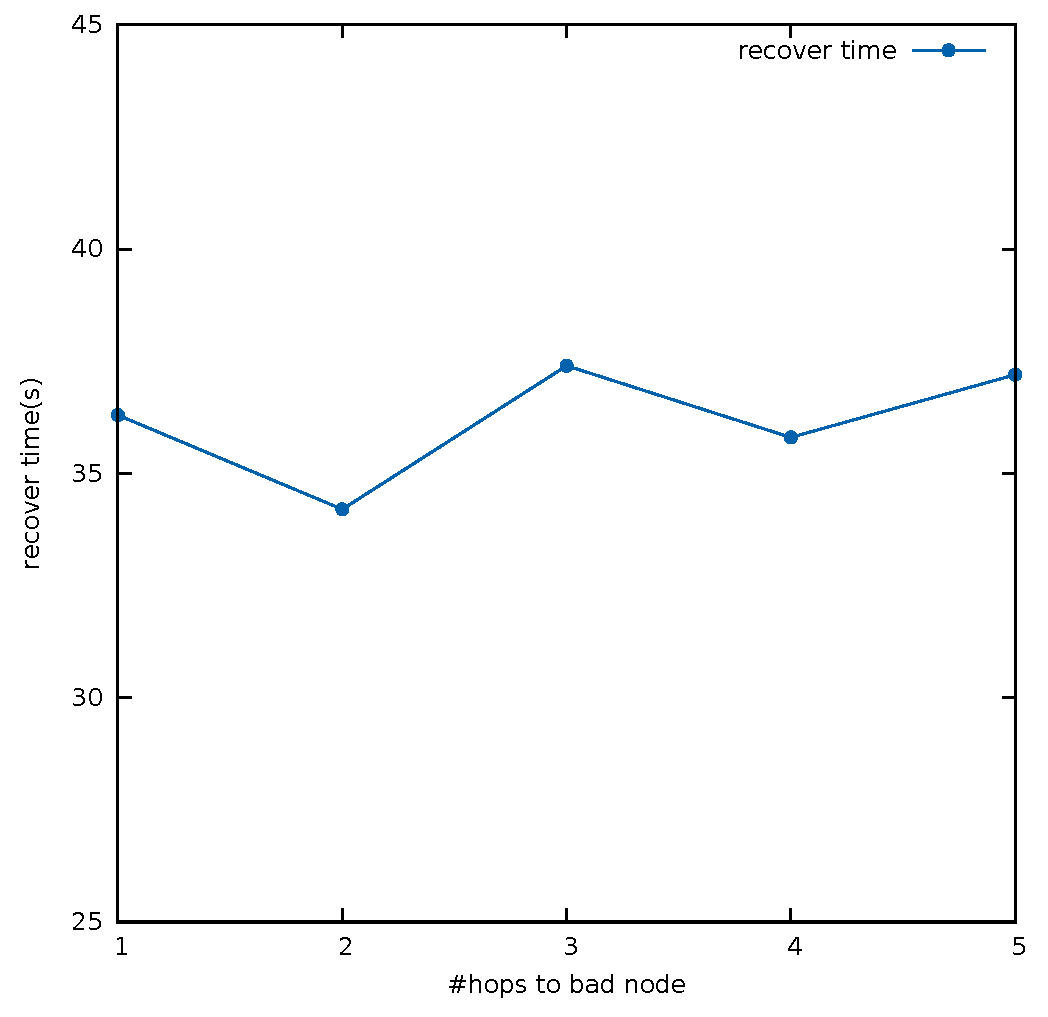
\includegraphics[scale=0.3]{pic/faultToleranceTime.eps}
\end{center}
\caption{Recovery time from faults}
\label{fig:faultTolerance}
\end{figure}

\begin{table}[h]
\begin{center}
\begin{tabular}{|l|l|}
\hline
Operation & Time (s) \\ \hline
failure detection & 24 \\ \hline
metadata server reschedule & 0.3 \\ \hline
closing old stream pipe & 1.2 \\ \hline
open new stream pipe & 1.3 \\ \hline
server buffering & 7.2 \\ \hline
client buffering & 2 \\ \hline
\end{tabular}
\caption{Recovery activity time}
\end{center}
\label{tab:recovery}
\end{table}


\section{Related Works}
\paragraph{Crowd-sourcing Video}
GigaSight~\cite{simoens2013scalable} is a framework for sharing crowd-sourcing videos. What it does is to store video data locally and upload metadata of the stream to the central server. When this video is requested by other users it will then upload the stream to the central video server and the user can watch it. It's more like a distributed video storage system. Our system is a distributed video streaming system and we do not have central video server. Since our system is designed for live streaming system, we do not need to store the data, we focused more on the bandwidth optimizations.
SignalGuru~\cite{koukoumidis2012leveraging} is a framework to use crowd-sourcing video streams to predict traffic lights transition times so as to improve accuracy in predicting arrival time. This framework could utilize our service to better utilize the WAN bandwidth. Another good use of crowd-sourcing video is Movi~\cite{bao2010movi}. It could automatically detect social hot points based on smartphone sensors. All these crowd-sourcing videos can use our decentralized streaming system as a network infrastructure.

\paragraph{Bandwidth Optimization}
One important assumption our system made is LAN is ample even it is wireless LAN. Currently, IEEE 802.11~\cite{crow1997ieee} is the most widely used wireless LAN protocol. The latest 802.11ac~\cite{ong2011ieee} reports an 1300 Mbps theoretical speed and gives us the confidence to make this assumption. Peer to peer is a popular strategy used to optimize utilization of the WAN bandwidth. Vivaldi~\cite{dabek2004vivaldi} optimized the latency prediction between two peers by constructing a coordinate system. ZIGZAG~\cite{tran2003zigzag} used a hierarchical structure for organizing peers and built a multicast tree based on the bounded-size clusters to make the tree flat. PROMISE~\cite{hefeeda2003promise} tries to do an automatic and intelligent network topology inference to get better performance. We used some of the ideas in those peer-to-peer work to build our overlay tree.

\paragraph{Video Streaming}
Video streaming has been studied for a long time in both academia and industry. Researchers have made big improvements on this area. Asit Dan has tried proposed a dynamic batching policy to batch requests and use multicast on routers to save data this server needs to send~\cite{dan1996dynamic, dan1994scheduling}. T. Nguyen proposed a new transport protocol which is receiver-driven to enable simultaneous transmissions of video from multiple senders. This way, they could achieve higher throughput for that receiver. AnySee~\cite{liao2006anysee} uses uses inter-overlay information to get global knowledge about the whole overlay network structure and so as to make better tree decisions to decrease latency. GridMedia~\cite{zhang2005large} uses a push-pull strategy to get packets. The traditional way is to just pull data. The pull-push way can reduce latency by server pushing more recent data to the clients.

\paragraph{Cloudlet}As M. Satyanarayanan said in 2013, "A cloudlet represents the middle tier of a 3-tier hierarchy: mobile device – cloudlet – cloud, and can be viewed as a data center in a box” whose goal is to bring the cloud closer"~\cite{satyanarayanan2013cloudlets}. Small computations can be finished on cloudlets and large computations will be pushed to the real cloud. That's the key principle of cloudlets. It can effectively reduce latency and suffer less from the Internet congestions and jitters. Cloudlet has soft states, low LAN latency and high LAN bandwidth~\cite{satyanarayanan2011mobile}, which makes it a perfect match to do application layer multicast. We used the vm based cloudlet proposed by M. Satyanarayanan~\cite{satyanarayanan2009case}.

\section{Future Work}
The work described here is a first try to build a decentralized video streaming system on cloudlets. It shows the benefits of using this decentralized model doing ALM. There are still several important parts that could be optimized.

\paragraph{Scheduling Algorithm}
Our system does scheduling based on the hops to root and the spare bandwidth on that cloudlet. This strategy will try to schedule a node with smallest latency and ample spare bandwidth. However, latency is not only determined by hops to the root. It's also related with network condition to the root and geographical position. To make a better scheduling decision, we need to use this kind of information to better schedule nodes and optimize the overlay tree structure.

\paragraph{Optimize latency}
Currently, latency is high for a client if it is tens or hundreds of hops away to the sender. Latency can be improved if we build our own streaming server. Latency mainly comes from the buffering in streaming server. This buffering is used for the streaming server to smoothly serve and and recognize incoming stream codec when it first receive the stream. If we use fixed codec for the streams in our system, we can reduce the buffer size and reduce the latency.

\section{Conclusion}
In this paper, we proposed a new decentralized live streaming model. This model will do application layer multicast on cloudlets and can greatly reduce WAN bandwidth consumption and solve the single point bandwidth bottleneck in a systematic way. We have implemented the system and tested its performance and showed its effectiveness. Our system is intended to be running at Internet scale and we anticipated various failures could occur. Our system can tolerate any kind of client failures and cloudlet failures. Besides, we used Google AppEngine with high replicated datastore to guarantee availability of the metadata server.

Better using WAN bandwidth is a hard problem and multicast is an accepted good way to deal with this problem. However, multicast on routers is not widely used for various technology and economy reasons. With the coming of cloudlets, we see a great opportunity to do multicast. It is on application layer so we do not need to change the network infrastructure. Besides, cloudlet is attached to the local access point, so using cloudlet to do application layer multicast is just like doing multicast on routers. We showed by building this system that cloudlets can be effectively used to better solve hard network problems in the old client-server model.

\section{My Contributions}
This work can be finished within three months is largely because of the valuable help from Zhuo Chen, Wolfgang Richter and developers of ffmpeg, libstreaming library on Android system and Nginx server.

Zhuo Chen gives me the initial idea of using cloudlets to build a decentralized streaming system and adaptively change the video resolution. He gives me much help on refining this idea, debugging Google Glass related programming problems and finding right tools to do streaming. Wolfgang Richter gives me great help on using Nginx server with rtmp module and provides me with the VM instances on WolfStack. I want to sincerely thank them here.

We used some open source libraries and tools in building the system and the demo client. We used libstreaming library~\cite{libstreaming} to encode video into h264 codec and borrowed example 1 of libstreaming tutorial to send streaming data to our streaming server. We used ffmpeg~\cite{tomar2006converting} to pipe the stream between different streaming servers. We used Nginx with rtmp module~\cite{nginx} as our streaming server. We used bootstrap~\cite{bootstrap} to build our demo website. Thanks all the developers of those open source tools and libraries. You made programmers' lives much easier.

My contribution in this work is to design and build the whole system. I came up with the idea of using application layer multicast on cloudlets. I designed the scheduling algorithm, fault tolerant protocol, all the meta data structure and database schema. I wrote all the codes on the cloudlets, stream monitor, metadata server, website and the communication part of Google Glass demo client code.

\section{Availability}

This work is completely open sourced. All the codes are available on github. Metadata server code is at

\begin{center}
 \emph {https://github.com/AnbangZhao/p2pMeta}\\
\end{center}

Cloudlet server, stream monitor and demo website code is at
\begin{center}
\emph {https://github.com/AnbangZhao/liveStreamingWeb}\\
\end{center}

Demo client code on Google Glass is at
\begin{center}
\emph {https://github.com/AnbangZhao/liveStreamingClient}\\
\end{center}


{\footnotesize \bibliographystyle{acm}
\bibliography{./bibliography/mybib}}



\end{document}






